% Created 2020-05-17 Sun 14:32
% Intended LaTeX compiler: pdflatex
\documentclass[unrestricted]{meetingnotesminutes}
                    \title{ {{{title}}} }
\author{ {{{author}}} }
\project{ {{{keyword(PROJECT)}}} }
\wheremeeting{ Teams }
\whenmeeting{ 17 May, 2020 }
\initiator{Vi Kumar}
\participant[present]{Abdullah Sherif - as394@hw.ac.uk}
\participant[present]{Vishakh Kumar - vpk2@hw.ac.uk}
\participant[present]{Vishnu Sarathy - vks2@hw.ac.uk}
\participant[information]{Dr Mehdi Nazarinia}
\participant[present]{Dr Ityonna Amber}
\date{}
\title{}
\hypersetup{
 pdfauthor={},
 pdftitle={},
 pdfkeywords={},
 pdfsubject={},
 pdfcreator={Emacs 26.3 (Org mode 9.3.6)},
 pdflang={English}}
\begin{document}

\frontmatter

\section{Agenda}
\label{sec:org300fc4e}
\section*{Agenda}
\begin{itemize}
  \item Housingkeeping \& Onboarding
  \item Current Status of Project
  \item Action items
\end{itemize}

\section{Housekeeping \& Onboarding}
\label{sec:org635cd19}
\subsection{New member!}
\label{sec:org669c370}
Vishnu Sarathy is our new member! Introduce yourself!

\subsection{Git Repository}
\label{sec:org767152c}
Get used to git because that's the easiest way for us to work together.
Great documentation at \url{https://git-scm.com/doc}

Quick reference:
\begin{verbatim}
git pull origin master
git add .
git commit -m "Useful message"
git push origin master

Our repo: https://gitlab.com/grokkingStuff/MathWorksMiniDrone
\end{verbatim}

\section{Current Status of Project}
\label{sec:org0dce987}
\subsection{Mission Timeline}
\label{sec:org0b276e1}
\textbf{Key feedback}:

\begin{itemize}
\item Test, test, test
Compare the ROS-model ORB-SLAM vs the Simulink model
IF it passes the stages, compare times.
Work w/ Vishnu \& Sheriff on this ASAP
\end{itemize}

\subsubsection{Time consideration?}
\label{sec:orgd9eb607}
Time consideration?
Time considered only when the minidrone lands on the end marker.

In order for the minidrone to be considered as having landed:
\begin{itemize}
\item Minidrone must be upright.
\item Minidrone's bottom surface has to touch the floor.
\end{itemize}
\begin{center}
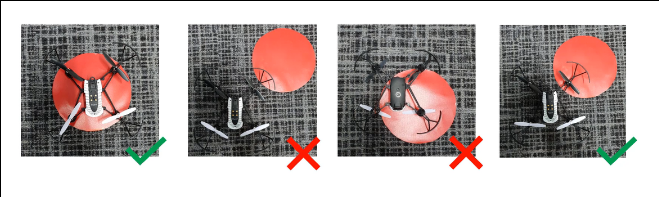
\includegraphics[width=.9\linewidth]{./images/screenshot-01.png}
\end{center}

\subsection{General Software Stack}
\label{sec:org7bbea01}
Work off ROS inside Simulink.

\begin{itemize}
\item Why?
\end{itemize}
Plenty of existing models in ROS that are industry-tested. Also, it's usually been optimized for the purpose and the ability to just subscribe to a node that gives you information is crazy useful

\begin{itemize}
\item So why Simulink?
\end{itemize}
The control logic is best expressed in Simulink because writing C code that has a decent state machine AND is able to interface with ROS nodes AND is able to help us out with a GUI/debug tools IS HARD! Simulink acts as a glue between our hardware, voodoo blackbox, and our ideas.

\subsubsection{Matlab/Simulink}
\label{sec:orgbed147f}
Not gonna write much here because I think everyone is familiar with it.

Status: Installed

\subsubsection{ROS}
\label{sec:org42eb7d0}
Robot Operating System (ROS) is a framework of tools, libraries, and software to aid in robot software development. It is a flexible system for programming robots and controlling robotic platforms. ROS was developed by an open-source collaborative community to help grow the world of robotics. Applications for working with hardware, robotic simulation models, path planning, localization and mapping, and many other algorithms are available. For an introduction to ROS, see the ROS Introduction on their website.

\begin{enumerate}
\item ROS Toolbox in Simulink
\label{sec:orgca215c6}

\url{https://www.mathworks.com/help/ros/gs/robot-operating-system-ros.html}

ROS Toolbox allows you to access ROS functionality in MATLAB®. Use MATLAB to communicate with a ROS network, interactively explore robot capabilities, and visualize sensor data. You can develop robotics applications by exchanging data with ROS-enabled robots and robot simulators such as Gazebo. You can also create Simulink® models that exchange messages with a ROS network. Verify your model within the Simulink environment by receiving messages from, and sending messages to, ROS-enabled robots and robot simulators. From your model, you can also generate C++ code for a standalone ROS application.

Both MATLAB and Simulink support the TCPROS transport layer (see TCPROS). The UDPROS transport is not supported.

ROS Toolbox supports ROS Indigo and Hydro platforms, but your own ROS installation may have different message versions. If you would like to overwrite our current message catalog, you can utilize ROS Custom Message Support to generate new message definitions. For ROS 2, ROS Toolbox supports the Dashing Diademata platform.
\end{enumerate}

\subsection{Control Scheme}
\label{sec:org327d897}
\subsubsection{Drone Finite State Machine}
\label{sec:org59c9b2f}
\begin{center}
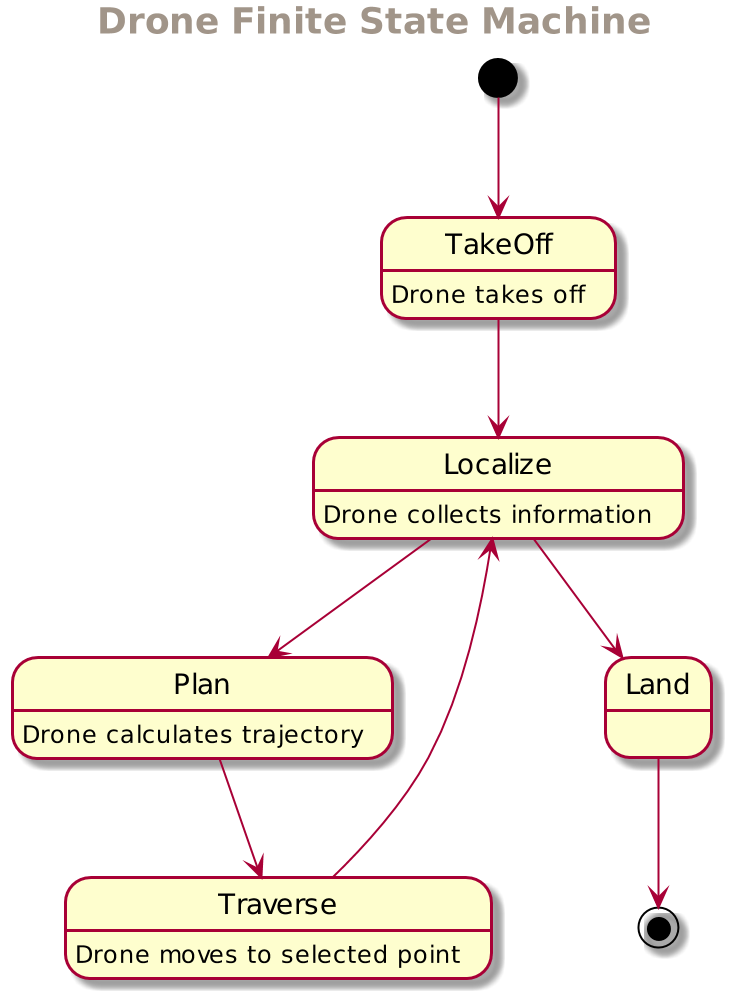
\includegraphics[width=.9\linewidth]{drone-fsm.png}
\end{center}



So our drone needs a way to figure out what to do and how to do it.
A really simple Finite State Machine is below. Should probably ask someone who knows what they're doing.

The SLAM algorithm is commputer intensive BUT once localization is done, it's pretty fast.

So our first pass will be super slow to collect info.
Then, we can use the state machine to switch between the Localize \& Traverse states and make optimal use of information.

\subsubsection{ORB-SLAM2}
\label{sec:orga5e2177}

\textbf{Status: Needs review}

Github-Repo: \url{https://github.com/raulmur/ORB\_SLAM2}

Youtube-Example: \url{https://www.youtube.com/watch?v=IuBGKxgaxS0}

ROS-Wiki Link: \url{http://wiki.ros.org/orb\_slam2\_ros}

License: GPLv3

\begin{quote}
ORB-SLAM2 is a real-time SLAM library for Monocular, Stereo and RGB-D cameras that computes the camera trajectory and a sparse 3D reconstruction (in the stereo and RGB-D case with true scale). It is able to detect loops and relocalize the camera in real time. We provide examples to run the SLAM system in the KITTI dataset as stereo or monocular, in the TUM dataset as RGB-D or monocular, and in the EuRoC dataset as stereo or monocular. We also provide a ROS node to process live monocular, stereo or RGB-D streams. The library can be compiled without ROS. ORB-SLAM2 provides a GUI to change between a SLAM Mode and Localization Mode, see section 9 of this document.
\end{quote}

\begin{enumerate}
\item ROS Parameters
\label{sec:org944c892}

There are three types of parameters right now: static- and dynamic ros parameters and camera settings from the config file. The static parameters are send to the ROS parameter server at startup and are not supposed to change. They are set in the launch files which are located at ros/launch. The parameters are:

\begin{itemize}
\item \texttt{load\_map}: Bool. If set to true, the node will try to load the map provided with map\textsubscript{file} at startup.
\item \texttt{map\_file}: String. The name of the file the map is saved at.
\item \texttt{settings\_file}: String. The location of config file mentioned above.
\item \texttt{voc\_file}: String. The location of config vocanulary file mentioned above.
\item \texttt{publish\_pose}: Bool. If a PoseStamped message should be published. Even if this is false the tf will still be published.
\item \texttt{publish\_pointcloud}: Bool. If the pointcloud containing all key points (the map) should be published.
\item \texttt{pointcloud\_frame\_id}: String. The Frame id of the Pointcloud/map.
\item \texttt{camera\_frame\_id}: String. The Frame id of the camera position.
\end{itemize}

Dynamic parameters can be changed at runtime. Either by updating them directly via the command line or by using rqt\textsubscript{reconfigure} which is the recommended way. The parameters are:

\begin{itemize}
\item \texttt{localize\_only}: Bool. Toggle from/to only localization. The SLAM will then no longer add no new points to the map.
\item \texttt{reset\_map}: Bool. Set to true to erase the map and start new. After reset the parameter will automatically update back to false.
\item \texttt{min\_num\_kf\_in\_map}: Int. Number of key frames a map has to have to not get reset after tracking is lost.
\end{itemize}

Finally, the intrinsic camera calibration parameters along with some hyperparameters can be found in the specific yaml files in orb\textsubscript{slam2}/config.

\item ROS Subscribed topics
\label{sec:org2778b5f}

\begin{itemize}
\item The \texttt{mono} node subscribes to \texttt{/camera/image\_raw} for the input image.
\item The RGBD node subscribes to \texttt{/camera/rgb/image\_raw} for the RGB image and
\item \texttt{/camera/depth\_registered/image\_raw} for the depth information.
\item The stereo node subscribes to \texttt{image\_left/image\_color\_rect} and
\item \texttt{image\_right/image\_color\_rect} for corresponding images.
\end{itemize}

\item ROS Published topics
\label{sec:org095f0d9}

The following topics are being published and subscribed to by the nodes:

\begin{itemize}
\item All nodes publish (given the settings) a PointCloud2 containing all key points of the map.
\item Live image from the camera containing the currently found key points and a status text.
\item A tf from the pointcloud frame id to the camera frame id (the position).
\end{itemize}

\item ROS Services
\label{sec:orgc107f8f}

All nodes offer the possibility to save the map via the service node\textsubscript{type}/save\textsubscript{map}. So the save\textsubscript{map} services are:

\begin{itemize}
\item \texttt{/orb\_slam2\_rgbd/save\_map}
\item \texttt{/orb\_slam2\_mono/save\_map}
\item \texttt{/orb\_slam2\_stereo/save\_map}
\end{itemize}
\end{enumerate}

\subsubsection{Unscented Kalman Filter}
\label{sec:org9c71e41}
\textbf{Status: Needs review}

Like an Extended Kalman Filter but more performant.
Able to deal with the drone's non-linearities and should give us a decent idea of where and how fast our drone is moving.

for the accelerometer, gyroscope and stuff
This is what keeps the drone actually flying in the air.
The ORB-SLAMv2 is really just a way to identify points

\section{{\bfseries\sffamily TODO} Action items}
\label{sec:orgdf38218}

\subsection{{\bfseries\sffamily TODO} Base Simulink Simulation}
\label{sec:org31c6ec2}
Also need to look at the base model (and add the existing stuff to git repo)

Some hard numbers instead of qualitative stuff.

\subsubsection{{\bfseries\sffamily TODO} Make comparison of models}
\label{sec:org4c5e95f}
\begin{itemize}
\item ROS vs Simulink
\item ORB-SLAM vs other vSLAM models
\item Different Feature Detection inside vSLAM
\end{itemize}

\subsubsection{{\bfseries\sffamily TODO} Simulink Model in Gitlab Repo}
\label{sec:org56feafc}
\begin{itemize}
\item[{$\square$}] Add the base case to the gitlab repo for convenience.
\item[{$\square$}] Notify Vishnu when done.
\end{itemize}

\subsubsection{Debugging}
\label{sec:org1bddf7b}

Useful link: \url{https://www.mathworks.com/matlabcentral/answers/?term=parrot}


\subsection{{\bfseries\sffamily TODO} ORB-SLAM Simulink model}
\label{sec:org1afff8e}
Implement ORB-SLAM in Simulink (again, ughh).

\subsection{{\bfseries\sffamily TODO} Need to get real-life data for stuff}
\label{sec:orgaa1723f}
Need to get Dr Mehdi to send over a recording of sensor data from the drone. While we can't actually work with said drone thanks to the whole lockdown, having some raw data should allow us to make (somewhat rational) decisions about which filters and what parameters to use to analyze said data.

Not a priority (yet) and I think Dr Mehdi is busy with exam stuff. Would recommend bugging him about it before our meeting on May 17.

\subsection{{\bfseries\sffamily TODO} Equations of motion}
\label{sec:orga13cdb2}
For the UKF because you need a proper statespace model

\subsubsection{Need some controlability analysis}
\label{sec:org1fa39f7}
Mostly so that we know we're not missing out on some really useful info.

Give Sheriff some equations to use the SVD analysis on
Two birds with one stone - Controllability analysis as well as practice for Sheriff.
\end{document}
